% =============================================================================
\chapter{Squeezing in BEC interferometry}
\label{cha:bec-squeezing}
% =============================================================================

As we have seen in the previous chapters, the truncated Wigner method provides significant corrections to such important experimental observables as visibility or phase noise.
While they do establish the theoretical limits for these quantities, real measurements are still mostly limited by technical noise, which do not require quasiprobability methods to account for.

In this chapter we will consider a property of \abbrev{bec} interferometry experiments which cannot be obtained from the mean-field approximation.
This property is the degree of spin squeezing, which allows to reduce the minimum uncertainty of the collective spin of a two-component \abbrev{bec} below the shot noise limit.
A state with a high degree of coherence between the two components, the coherent spin state~\cite{Kitagawa1993}, has equal uncertainty in any direction.
Further evolution and nonlinear interactions can redistribute quantum noise, making it possible to achieve an uncertainty lower than the shot noise along one direction (at the price of the increased uncertainty in other directions, to preserve the Heisenberg inequality).
Spin squeezing has been theoretically introduced by Kitagawa and Ueda~\cite{Kitagawa1993}, and by Wineland \textit{et~al}~\cite{Wineland1994}, and later observed experimentally~\cite{Hald1999,Kuzmich2000}.
It allows an outcome of interferometry experiments to be measured with uncertainty beyond the standard shot noise limit~\cite{Riedel2010,Gross2010} and can serve as a measure of entanglement in a two-component \abbrev{bec}~\cite{Sorensen2001,He2012a}.

In this chapter we will derive an expression that will allow us to obtain the degree of squeezing from the moments of wavefunctions in the truncated Wigner method, and apply it to a recent spin squeezing experiment.
We will also consider another possible experiment with a \abbrev{bec} near a Feshbach resonance where spin squeezing can be observed and discuss the complications caused by nonlinear losses.


% =============================================================================
\section{Spin squeezing in the Wigner representation}
\label{sec:bec-squeezing:theory}
% =============================================================================

Following S{\o}rensen \textit{et~al}~\cite{Sorensen2001} and Li \textit{et~al}~\cite{Li2009}, we define the components of the spin vector $\hat{\mathbf{S}} \equiv (\hat{S}_x, \hat{S}_y, \hat{S}_z)$ in terms of field operators as
\begin{eqn}
	\hat{S}_x
	& = \frac{1}{2} \int \upd \xvec \left(
			\Psiop_2^\dagger \Psiop_1 + \Psiop_1^\dagger \Psiop_2
		\right), \\
	\hat{S}_y
	& = \frac{i}{2} \int \upd \xvec \left(
			\Psiop_2^\dagger \Psiop_1 - \Psiop_1^\dagger \Psiop_2
		\right), \\
	\hat{S}_z
	& = \frac{1}{2} \int \upd \xvec \left(
			\Psiop_1^\dagger \Psiop_1 - \Psiop_2^\dagger \Psiop_2
		\right).
\end{eqn}
The degree of squeezing is then
\begin{eqn}
\label{eqn:bec-squeezing:theory:xi2}
    \xi^2
    = \frac{N \min_{\vec{n} \perp \hat{\langle \mathbf{S} \rangle}} \Delta \hat{S}^2_{\vec{n}}}%
    	{\langle \hat{\mathbf{S}} \rangle^2},
\end{eqn}
where $\Delta \hat{S}^2_{\vec{n}}$ is the variance of the total spin along the direction $\vec{n}$, and $N$ is the total number of atoms.
This quantity can serve as an entanglement criterion, indicating its occurrence when $\xi^2 < 1$~\cite{Sorensen2001}.
Note that in this thesis we only consider the squeezing along the direction orthogonal to the total spin, as was originally introduced, but other definitions are also possible~\cite{He2011}.

A straightforward way of finding the $\xi^2$ is to shift the coordinate frame to the end of the vector $\langle \hat{\mathbf{S}} \rangle$, and rotate it so that one of the axes is aligned along it.
The minimum variance can then be found by varying the angle of rotation of the other two axes and calculating the variance along one of them (in fact, this is how it is usually done in the experiment).
The direct approach consists of expressing the desirable minimum variance in terms of variances of the components of the spin vector in the original coordinates~\cite{Li2009}.
We denote the polar and the azimuthal angle of $\langle \hat{\mathbf{S}} \rangle$ as $\nu$ and $\phi$ respectively, meaning that
\begin{eqn}
	\nu = \arccos \frac{\langle \hat{S}_z \rangle}{\langle \hat{\mathbf{S}} \rangle},\quad
	\phi = \arg \langle \hat{S}_x + \hat{S}_z \rangle.
\end{eqn}
The minimum uncertainty is then expressed as
\begin{eqn}
	\min_{\vec{n} \perp \langle \hat{\mathbf{S}} \rangle} \Delta \hat{S}^2_{\vec{n}}
	={} & \frac{1}{2} \left(
			\cos^2 \nu \cos^2 \phi + \sin^2 \phi
		\right) \Delta_{xx}
		+ \frac{1}{2} \left(
			\cos^2 \nu \sin^2 \phi + \cos^2 \phi
		\right) \Delta_{yy} \\
		& + \frac{1}{2} \sin^2 \nu\, \Delta_{zz}
			- \frac{1}{2} \sin^2 \nu \sin2\phi\, \Delta_{xy}
			- \frac{1}{2} \sin2\nu \cos \phi\, \Delta_{xz} \\
		& - \frac{1}{2} \sin2\nu \sin \phi\, \Delta_{yz}
		- \frac{1}{2} \sqrt{\tilde{A}^2 + \tilde{B}^2},
\end{eqn}
where
\begin{eqn}
	\tilde{A}
	={} & \left( \sin^2 \phi - \cos^2 \nu \cos^2 \phi \right) \Delta_{xx}
			+ \left( \cos^2 \phi - \cos^2 \nu \sin^2 \phi \right) \Delta_{yy} \\
		& - \sin^2 \nu\, \Delta_{zz}
			- \left( 1 + \cos^2 \nu \right) \sin2\phi\, \Delta_{xy} \\
		& + \sin2\nu \cos \phi\, \Delta_{xz}
			+ \sin2\nu \sin\phi\, \Delta_{yz},
\end{eqn}
and
\begin{eqn}
	\tilde{B}
	={} & \cos\nu \sin2\phi \left( \Delta_{xx} - \Delta_{yy} \right)
			- 2 \cos\nu \cos2\phi\, \Delta_{xy} \\
		& - 2 \sin\nu \sin\phi\, \Delta_{xz}
			+ 2 \sin\nu \cos\phi\, \Delta_{yz}.
\end{eqn}
The spin correlations $\Delta_{ij}$ are defined as
\begin{eqn}
	\Delta_{ij}
	= \frac{1}{2} \langle \hat{S}_i \hat{S}_j + \hat{S}_j \hat{S}_i \rangle
		- \langle \hat{S}_i \rangle \langle \hat{S}_j \rangle,\quad
		i,j=x,y,z.
\end{eqn}

Averages of the total spin vector components and their pairwise moments can be expressed calculated using moments of the Wigner functional according to~\eqnref{wigner-bec:fpe-bec:moments}.
The averages are calculated straightforwardly if we remember that the field operators of different components commute:
\begin{eqn}
	\langle \hat{S}_x \rangle
		& = \pathavg{\Real \int \Psi^*_1 \Psi_2 \upd\xvec }
		\equiv \pathavg{\Real I}
		\equiv \pathavg{S_x}, \\
	\langle \hat{S}_y \rangle
		& = \pathavg{\Imag \int \Psi^*_1 \Psi_2 \upd\xvec }
		\equiv \pathavg{\Imag I}
		\equiv \pathavg{S_y}, \\
	\langle \hat{S}_z \rangle
		& = \frac{1}{2} \pathavg{\int \Psi^*_1 \Psi_1 \upd\xvec - \int \Psi^*_2 \Psi_2 \upd\xvec}
		\equiv \pathavg{(N_1 - N_2) / 2}
		\equiv \pathavg{S_z},
\end{eqn}
where we have introduced the functionals of wavefunctions in a single simulation path $I \equiv S_x + i S_y$ and $(N_1 - N_2) / 2 \equiv S_z$.

The second-order moments of the spin operators are obtained by transforming normally ordered field operator products to symmetrically ordered ones, substituting path averages of wavefunction moments and grouping terms.
Starting with $\langle \hat{S}^2_x \rangle$, we can express it in terms of symmetrically ordered operator products as
\begin{eqn}
	\langle \hat{S}^2_x \rangle
	={} & \frac{1}{4} \left\langle \int
		\left(
			\Psiop^\dagger_2 \Psiop_1 + \Psiop^\dagger_1 \Psiop_2
		\right)
		\left(
			\Psiop^{\prime\dagger}_2 \Psiop^\prime_1 + \Psiop^{\prime\dagger}_1 \Psiop^\prime_2
		\right)
		\upd\xvec\, \upd\xvec^\prime \right\rangle \\
	={} & \frac{1}{4} \left\langle \int \left(
			\symprod{ \Psiop^\dagger_2 \Psiop_1 \Psiop^{\prime\dagger}_2 \Psiop^\prime_1 }
			+ \symprod{ \Psiop^\dagger_1 \Psiop_2 \Psiop^{\prime\dagger}_2 \Psiop^\prime_1 }
		\right. \right. \\
		& \left. \left.
			+ \symprod{ \Psiop^\dagger_1 \Psiop_2 \Psiop^{\prime\dagger}_1 \Psiop^\prime_2 }
			+ \symprod{ \Psiop^\dagger_2 \Psiop_1 \Psiop^{\prime\dagger}_1 \Psiop^\prime_2 }
		\right. \right. \\
	& \left. \left.
		- \frac{1}{2} \Real \left(
			\delta_{\restbasis_1} (\xvec, \xvec^\prime)
			\delta_{\restbasis_2} (\xvec^\prime, \xvec)
		\right)
	\right) \upd\xvec\, \upd\xvec^\prime \right\rangle.
\end{eqn}
In general, basis sets of the first and the second component are different, and the last term in the above equation cannot be simplified any further.
However, in the numerical simulations in this chapter we use the same set $\restbasis_1 = \restbasis_2 = \restbasis$ for both components, which allows us to transform it to a more convenient form
\begin{eqn}
	\int \Real \left(
			\delta_{\restbasis} (\xvec, \xvec^\prime)
			\delta_{\restbasis} (\xvec^\prime, \xvec)
		\right) \upd\xvec\, \upd\xvec^\prime
	& = \frac{1}{2} \int \left(
			\sum_{\mvec \in \restbasis} \phi_{\mvec}^\prime \phi_{\mvec}^*
			\sum_{\nvec \in \restbasis} \phi_{\nvec} \phi_{\nvec}^{\prime*}
			+ \mathrm{c.\,c.}
		\right) \upd\xvec \upd\xvec^\prime \\
	& = \frac{1}{2} \sum_{\mvec \in \restbasis} \sum_{\nvec \in \restbasis}
		\left(
			\delta_{\mvec,\nvec} \delta_{\mvec,\nvec}
			+ \delta_{\mvec,\nvec} \delta_{\mvec,\nvec}
		\right) \\
	& = | \restbasis |,
\end{eqn}
where we have expanded the restricted delta functions using the expression from \defref{func-calculus:restricted-delta}.
Applying~\eqnref{wigner-bec:fpe-bec:moments} to the full expression for $\langle \hat{S}^2_x \rangle$, we rewrite it in terms of wavefunctions in the Wigner representation:
\begin{eqn}
	\langle \hat{S}^2_x \rangle
	& = \frac{1}{4} \pathavgleft
		\int \Psi^*_2 \Psi_1 d\xvec \int \Psi^*_2 \Psi_1 d\xvec
		+ \int \Psi^*_1 \Psi_2 d\xvec \int \Psi^*_2 \Psi_1 d\xvec \right. \\
	&	\left. + \int \Psi^*_1 \Psi_2 d\xvec \int \Psi^*_1 \Psi_2 d\xvec
		+ \int \Psi^*_2 \Psi_1 d\xvec \int \Psi^*_1 \Psi_2 d\xvec
		- \frac{|\restbasis|}{2} \pathavgright \\
	& = \frac{1}{4} \pathavg{ (I^*)^2 + I I^* + I^2 + I^* I } - \frac{|\restbasis|}{8} \\
	& = \pathavg{ (\Real I)^2 } - \frac{|\restbasis|}{8}
	= \pathavg{ S^2_x } - \frac{|\restbasis|}{8}.
\end{eqn}

Using the same procedure, we find the expectations for other pairwise moments of the spin operators:
\begin{eqn}
	\langle \hat{S}^2_y \rangle
	& = \pathavg{ S^2_y } - \frac{|\restbasis|}{8}, \\
	\langle \hat{S}^2_z \rangle
	& = \pathavg{ S^2_z } - \frac{|\restbasis|}{8}, \\
	\frac{1}{2} \langle \hat{S}_x \hat{S}_y + \hat{S}_y \hat{S}_x \rangle
	& = \pathavg{ S_x S_y }, \\
	\frac{1}{2} \langle \hat{S}_x \hat{S}_z + \hat{S}_z \hat{S}_x \rangle
	& = \pathavg{ S_x S_z }, \\
	\frac{1}{2} \langle \hat{S}_y \hat{S}_z + \hat{S}_z \hat{S}_y \rangle
	& = \pathavg{ S_y S_z }.
\end{eqn}

Now we have all the required expectations to calculate the spin correlations $\Delta_{ij}$ and, consequently, the degree of squeezing $\xi^2$.
Note that if we neglect the term $|\restbasis|/8$ in the equations for $\langle \hat{S}_i^2 \rangle$ (which is small as compared to $S_i^2$ when the Wigner truncation condition~\eqnref{wigner-bec:truncation:delta-condition} applies), the spin correlations behave ``classically''.
This means that they behave as if we had a ``cloud'' of spin vectors, where each vector corresponds to a separate simulation path, and the correlations are classical correlations of different vector components in this cloud.
Consequently, without giving up too much accuracy we can informally illustrate the total spin uncertainty by plotting the distribution of the total spin vector $(S_x, S_y, S_z)$ over the integration trajectories.

% =============================================================================
\section{Squeezing by component separation}
% =============================================================================

As an example of measurement of the degree of squeezing in a real two-component \abbrev{bec} system, we will consider a recent experiment~\cite{Riedel2010}, in which multi-particle entanglement and resulting spin squeezing was achieved with the help of component-dependent potential.

The experiment essentialy consisted of the same regular Ramsey sequence as depicted in~\figref{bec-noise:visibility:sequences},~(a) performed on $1250$ \Rb{} atoms in the hyperfine state ${\ket{F=1,\, m_F=-1}}$ in a cigar-shaped trap with $f_x = f_y = 109\un{Hz}$, $f_z = 500\un{Hz}$.
The experiment started with the application of a $\pi/2$-pulse using an oscillator with the Rabi frequency $\Omega=2.1\un{kHz}$, creating an equal superposition of two hyperfine states ${\ket{F=1,\, m_F=-1}}$ and ${\ket{F=2,\, m_F=+1}}$.
The second pulse had varied length allowing a measurement of the spin along the angle $\theta$: $\hat{S}_\theta = \hat{S}_z \cos \theta - \hat{S}_y \sin \theta$ (spin tomography).

The imporant difference was an addition of the component-dependent longitudinal shift to the potential $l_x = \pm 0.26\un{\mu m}$ right after the first pulse (as described by~\eqnref{bec-noise:system:V}), persisting the whole time of the evolution until the second oscillator pulse.
This effectively reduced the component overlap and provided a way of controlling the nonlinearity and the spin squeezing according to the ``one-axis twisting Hamiltonian'' model~\cite{Kitagawa1993}.

\begin{figure}
    \centerline{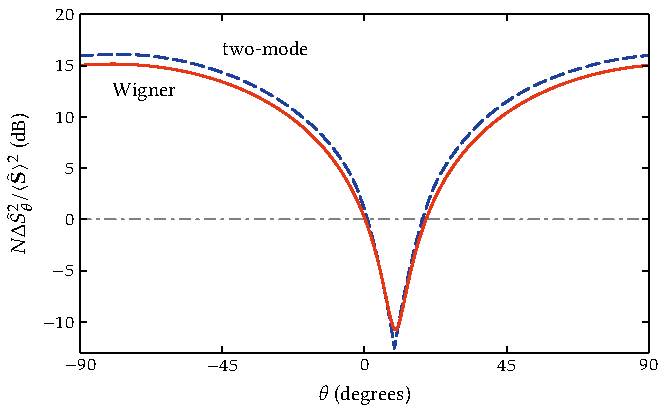
\includegraphics{figures_generated/bec_squeezing/riedel_rotation.pdf}}

    \caption{
    The dependence of the normalized variance on the rotation angle $\theta$ for the Wigner method (red solid line) and the two-mode variational method (dashed blue line, data taken from~\cite{Riedel2010}).
    }
    \label{fig:bec-squeezing:separation:tomography}
\end{figure}

The truncated Wigner approach is applied straightforwardly to this system and allows us to measure the degree of squeezing $xi^2$ according to the formula~\eqnref{bec-squeezing:theory:xi2}, calculating the required spin correlations using the expressions derived in \secref{bec-squeezing:theory}.
Furthermore, we can simulate the observations closer to those used in the experiment, and collect the spin tomography results, as shown in~\figref{bec-squeezing:separation:tomography}.
The maximum degree of squeezing and the corresponding rotation angle corresponds to the minimum of the graph.

The Wigner method shows good agreement with the two-mode variational method~\cite{Li2009}, which was used by the experimental team, and also includes the effect of particle losses.
The two-mode method predictions were taken from~\cite{Riedel2010} and plotted in~\figref{bec-squeezing:separation:tomography} for the sake of comparison \todo{can we do that?}.
The figure demonstrates that the predictions of the two methods for the maximum squeezing angle are nearly identical, and the predictions of the degree of squeezing are close, yet noticeable different ($-10.73\pm0.05\un{dB}$ from the Wigner method as compared with $-12.8\un{dB}$ from the two-mode method).
We believe this is caused by the Wigner method being a more systematic type of approximation with a small parameter, and consequently, more suitable for such complex calculations.

This prediction is hard to verify experimentally, as the technical noise greatly reduces the degree of squeezing (down to $-3.7\un{dB}$), moving it far from the theoretical limit.
The technical noise was not included in the simulations in this thesis, although it can be done similarly to \charef{bec-noise} (since the techincal noise in this experiment has the same nature).
On the other hand, the maximum ``unsqueezing'' (the maximums of the plot in~\figref{bec-squeezing:separation:tomography}), while being irrelevant for practical purposes, can serve as a good experimental check for the two-mode and Wigner methods, as it is much less affected by the technical noise.
The difference of $1\un{dB}$ in the maximum unsqueezing between the two methods should be possible to distinguish.

\begin{figure}
    \centerline{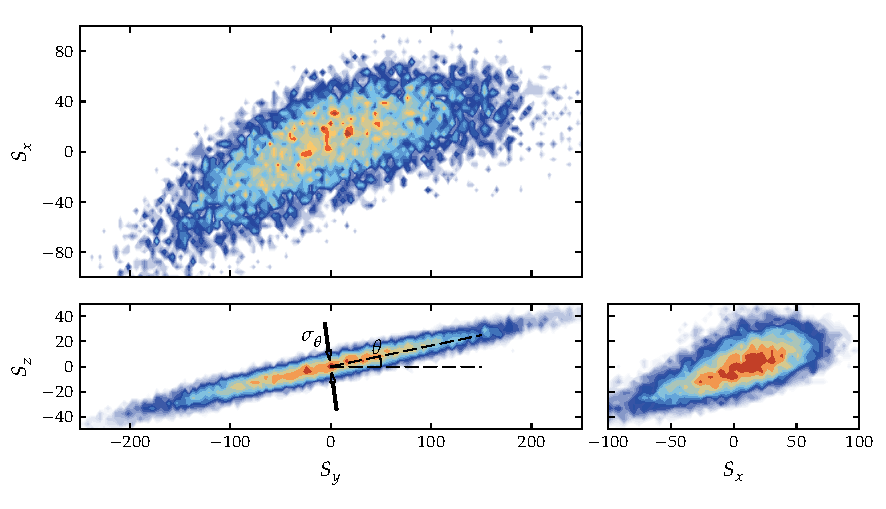
\includegraphics{figures_generated/bec_squeezing/riedel_cloud.pdf}}

    \caption{
    Reconstructed probability distribution for the value of the spin vector projected on $y,z$ plane (a) and spin noise tomography (b).
    The variance $\Delta^2 \hat{S}_\theta$ is connected to the width of the distribution $d_\theta$ in direction $\theta$ (blue line between two arrows in panel (a)) as $2 \sqrt{\Delta^2 \hat{S}_\theta} = d_\theta$.}
    \label{fig:bec-squeezing:separation:cloud-yz}
\end{figure}

We can go further and reconstruct the spin noise distribution using the per-path values of the total spin components, as explained in the end of \secref{bec-squeezing:theory}.
The uncertainty of the total spin in the orthogonal plane is shown in~\figref{bec-squeezing:separation:cloud-yz}.
The shape of the cloud is similar to the one obtained experimentally~\cite{Riedel2010}, and it also serves as a good illustration of the physical meaning of the maximum degree of squeezing and the corresponding rotation angle.

It is interesting to look at all three projections of the cloud, shown in~\figref{bec-squeezing:separation:cloud-yz}.
It is clearly seen that indeed the direction used to measure the squeezing in the experiment is indeed the best one, and the cloud is much wider in other directions.

% =============================================================================
\section{Squeezing near a Feshbach resonance}
% =============================================================================

In the previous section we have discussed an experiment where squeezing was achieved with component-dependent potentials, which helped to reduce the inter-component interaction.
The same effect can be achieved differently~--- by manipulating the external magnetic field near a Feshbach resonance for a chosen pair of hyperfine states.
This allows one to vary the interaction in a wide range with relative ease.
The downside of this approach is a significant increase of the inter-component nonlinear loss rate accompanying the change in the interaction strength.
This results in the destruction of the squeezing as the two components interfere with each other and lose coherence.

The truncated Wigner approach allows us to investigate the combined effect of a reduced interaction strength and increased losses.
In this section we will consider a hypothetical interferometry experiment with two hyperfine states of \Rb{} and demonstrate how with the help of the Wigner method we can pick the optimal value of the magnetic field that leads to the maximum squeezing.

The experiment follows the general scheme used in this and the previous chapters.
We start from a \abbrev{bec} of $N = 55000$ \Rb{} atoms in the hyperfine state ${\ket{F=1,\, m_F=+1}}$ in a cigar-shaped trap with the frequencies $f_x = f_y = 97.0\un{Hz}$ and $f_z = 11.69\un{Hz}$.
The first $\pi/2$-pulse creates an equal superposition of two states, ${\ket{F=1,\, m_F=+1}}$ and ${\ket{F=2,\, m_F=-1}}$.
The external magnetic field of strength $B \approx B_0$ is applied, where $B_0 = 9.1047\un{G}$ corresponds to the Feshbach resonance for the two hyperfine states used~\cite{Kaufman2009}.
We then investigate the time dependence of the maximum degree of spin squeezing.
Intra-component interaction strengths do not depend on the external magnetic field, and are taken to be $a_{11} = 100.4\,r_B$ and $a_{22} = 95.44\,r_B$.

The dependence of the inter-component interaction and loss rate can be described with a single equation for the complex scattering length~\cite{Kaufman2009}
\begin{eqn}
    a(B)
    = a_{\mathrm{bg}} \left(
        1 - \frac{\Delta B}{(B - B_0) - i \gamma_B / 2}
        \right),
\end{eqn}
where $a_{\mathrm{bg}}$ is the background scattering length, $\Delta B$ is the resonance width, and $\gamma_B$ is the decay width.
For a given $B$, the real part of this value acts as the $s$-wave scattering length $a_{12}$ in~\eqnref{bec-noise:system:g}:
\begin{eqn}
\label{eqn:bec-squeezing:feshbach:g}
    g_{12}(B)
    = \frac{4 \pi \hbar^2 \Real a(B)}{m}
    = \frac{4 \pi \hbar^2 a_{\mathrm{bg}}}{m} \left(
        1 - \frac{\Delta B (B - B_0)}{(B - B_0)^2 + \gamma_B^2 / 4}
    \right),
\end{eqn}
and the imaginary part can be connected to the loss rate by substituting it into~\eqnref{bec-noise:system:g} as well and comparing the resulting expression with the corresponding loss term in~\eqnref{bec-noise:mean-field:cgpes-simplified}:
\begin{eqn}
\label{eqn:bec-squeezing:feshbach:gamma}
    \gamma_{12}(B)
    = -\frac{8 \pi \hbar \Imag a(B)}{m}
    = \frac{4 \pi \hbar a_{\mathrm{bg}} \Delta B \gamma_B}{(B - B_0)^2 + \gamma_B^2 / 4}.
\end{eqn}

\begin{figure}
    \centerline{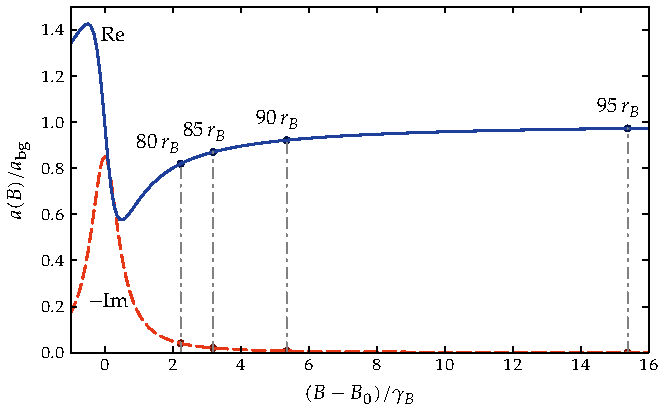
\includegraphics{figures_generated/bec_squeezing/feshbach_scattering.pdf}}

    \caption[Inter-component scattering lenth and loss rate near a Feshbach resonance]{
    Real (blue solid line) and imaginary (red dashed line, negated value is plotted for compactness) parts of the complex scattering length near the Feshbach resonance at $B_0 = 9.1047\un{G}$.
    Four pairs of points show the distances from the resonance chosen for the simulation.
    }%endcaption

    \label{fig:bec-squeezing:feshbach:scattering}
\end{figure}

For the Feshbach resonance we use the reported parameters are $\Delta B = 2\times10^{-3}\un{G}$, $\gamma_B = 4.7\times10^{-3}\un{G}$, and $a_{\mathrm{bg}} = 97.7\,r_B$~\cite{Kaufman2009}.
The behavior of the real and imaginary parts of $a(B)$ near the resonance is shown in~\figref{bec-squeezing:feshbach:scattering}.
From the equations above, as well as from the figure, it is obvious that the minimum inter-species scattering length is achieved when $B - B_0 = 0.5 \gamma_B$.
Unfortunately, this value also corresponds to a relatively large value of the imaginary part, and, correspondingly, the loss rate.
Therefore, we pick the values of $B$ further from the resonance, as displayed in the figure, where the interaction is somewhat stronger, but the loss rate is much lower.
The equations~\eqnref{bec-squeezing:feshbach:g} and~\eqnref{bec-squeezing:feshbach:gamma} give us the following values for the simulation:
\begin{eqn}
    B - B_0 & = 2.24 \gamma_B, \quad
        a_{12} = 80.0\,r_B, \quad \gamma_{12} = 3.85\times10^{-12}\un{cm^3/s},\\
    B - B_0 & = 3.20 \gamma_B, \quad
        a_{12} = 85.0\,r_B, \quad \gamma_{12} = 1.93\times10^{-12}\un{cm^3/s},\\
    B - B_0 & = 5.35 \gamma_B, \quad
        a_{12} = 90.0\,r_B, \quad \gamma_{12} = 7.00\times10^{-13}\un{cm^3/s},\\
    B - B_0 & = 15.4 \gamma_B, \quad
        a_{12} = 95.0\,r_B, \quad \gamma_{12} = 8.53\times10^{-14}\un{cm^3/s}.
\end{eqn}

\begin{figure}
    \centerline{%
    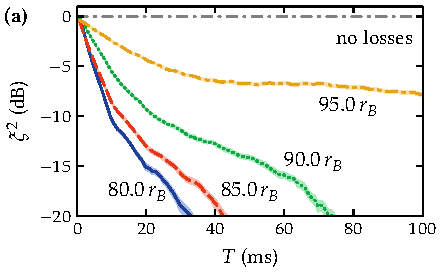
\includegraphics{figures_generated/bec_squeezing/feshbach_squeezing_no_losses.pdf}%
    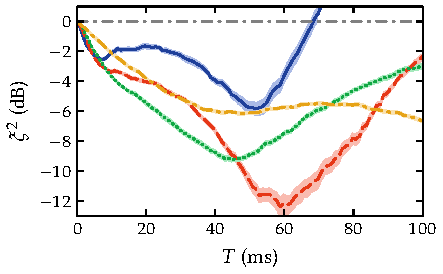
\includegraphics{figures_generated/bec_squeezing/feshbach_squeezing.pdf}}

    \caption[Spin squeezing near a Feshbach resonance]{
    Truncated Wigner simulations of the squeezing in the vicinity of the $B_0 = 9.1047\un{G}$ Feshbach resonance in \Rb{} with different values of the external magnetic field, with \textbf{(a)}~losses turned off, and \textbf{(b)}~inter-component $1,2$-losses turned on.
    Results corresponding to the scattering lengths $a_{12}=80.0\,r_B$ (blue solid line), $a_{12}=85.0\,r_B$ (red dashed line), $a_{12}=90.0\,r_B$ (green dotted line), and $a_{12}=95.0\,r_B$ (yellow dash-dotted line) are plotted.
    The same-colored bands show the estimated sampling error.}%endcaption

    \label{fig:bec-squeezing:feshbach:squeezing}
\end{figure}

First, we perform the simulations with $\gamma_{12}$ set to zero in order to test the squeezing in ideal conditions.
As expected, the lower $a_{12}$ is, the stronger squeezing is reachable, as shown in~\figref{bec-squeezing:feshbach:squeezing},~(a).

With the inclusion of the inter-component losses, the picture is different.
Feshbach tuning to $a_{12} = 85.0\,r_B$ ensures the best squeezing of the four variants ($-12\un{dB}$ at $60\un{ms}$), whereas long lasting squeezing is predicted for the variant with $a_{12} = 95.0\,r_B$ (\figref{bec-squeezing:feshbach:squeezing},~(b)).
In practice, it is possible to run the simulation for other values of $B$, thus finding the ideal balance between the interaction strength and the loss rate which produces the maximum squeezing.

% =============================================================================
\section{Conclusion}
% =============================================================================

In this chapter we have seen that the truncated Wigner approach can be successfully used to obtain correlations of the higher orders from the simulations without changing said simulations themselves, but only by processing the raw results.
Nonlinear elastic and inelastic interactions, along with various sources of technical noise can be added to the model straightforwardly, without affecting the measurement of the required correlations.
The Wigner method provides a solid framework for describing \abbreb{bec} interferometry experiments in cases when the density of a \abbrev{bec} stays high enough to satisfy the applicability condition~\eqnref{wigner-bec:truncation:delta-condition} (which is very often the case).

